\chapter{ケーススタディ:配列アラインメント}
本章では,生物学の分野において注目されている生物配列(DNAの塩基配列とタンパク質アミノ酸配列) の文字列処理(配列情報解析) 
\cite{浅井潔2000配列情報と確立モデル,後藤修1998マルチプルアラインメントは生体高分子情報の交差点}の中でも,配列アラインメントに焦点を当てる.
配列アラインメントの説明を行い,その後に配列アラインメント用の光Race Logic回路での設計選択肢を整理する.
その整理を基に,回路を提案する.

\section{配列アラインメントの基本原理}
DNAやタンパク質はユニットと名付けられた単位の物質が一列に並んだ高分子である.
ここでいうユニットとは,DNAにおいては4種の核酸,タンパク質においては20種類のアミノ酸である.
それぞれのユニットを文字としDNAやタンパク質の配列を単なる文字列だとみなして
処理をしてもある種の本質は失われないという考えに基づき,
文字列処理をすることで生物配列の解析を行なっている.
DNAの塩基配列やタンパク質アミノ酸配列の研究は,
バイオインフォマティクスの最重要課題の一つとして取り組まれてきた.
配列情報解析の重要な対象であるゲノム塩基配列は,
すでに200種類以上が決定されており,さらに多くの解析が進行中であるといわれている
\cite{浅井潔2005バイオインフォマティクス}.
生物配列の文字列処理の中で,DNA配列中に同じ順序で並んでいるユニットのパターンを見つける
配列アラインメントがある\cite{須戸里織2011バイオインフォマティクスゲノム配列から機能解析へバイオインフォマティクスゲノム配列から機能解析へ}.
アラインメントとは,複数の配列を入力として配列要素の間に最適な対応関係を求める処理であり,
配列の類似性判定に応用できるものである.
配列アラインメントの中でも,2つの配列間の類似性を判定する操作はペアワイズアラインメントと呼ばれ,
動的計画法による解法としてSW(Smith-Waterman)アルゴリズム\cite{smith1981identification}が存在する.
配列アラインメントは生物学において重要な手法であり,
計算機を用いた処理の高速化は従来よく多くの研究がなされてきた\cite{須戸里織2011gpu,宗川裕馬2008統合開発環境,sandes2011smith,liu2015accelerating,伊野文彦2007gpu}.

文字列の類似度を知るための典型的な手法は,情報理論に由来する編集距離である.
編集距離は具体的に,一文字の挿入・削除・置換によって一方の文字列をもう一方の文字列に変形するのに必要な手順の最小回数として定義される.
編集距離を理解するために,長さN = 5の文字列A= "TCGAT"と長さM = 5の文字列B= "GTCAC"を考える.
図\ref{dammy}は,文字列AをBに変換する2つの方法を示している.
上の行のスペースは挿入を表し,下の行のスペースは削除を表す.
両方の行に同じ文字がある列は一致,異なる文字がある列は不一致と呼ぶ.
特に、図\ref{dammy}の方法は文字GとTを削除し,GとCを挿入する一方で,図\ref{dammy}の方法は文字列Pを完全に削除して文字列Qを挿入している.

図\ref{dammy}および\ref{dammy}は, 2つのアラインメント方法の代替表現である.
任意の位置の数字は,図\ref{dammy}および\ref{dammy}の方法においてその位置までに存在する記号の数を示す.
この表示は各列の数値が図\ref{dammy}に示す編集グラフを構成する2次元N×Mグリッド内の座標と考えることができ,整列マトリックスとして知られている.
編集グラフは2つの文字列間において,取りうる限りの配置の2次元表現である有向非循環グラフ(DAG)である.
任意のアライメントは,すべてのエッジが編集操作に対応するこのグラフのパスで表現できる.
編集グラフの中の矢印は,可能なすべてのアライメントを示しており,
垂直の矢印は挿入を,水平の矢印は削除を,斜めの矢印一致を表している.
例えば、図\ref{dammy}の青と赤の矢印は,それぞれ図\ref{dammy}および\ref{dammy}に示す2つの特定のアライメントに対応している.

任意の2つの文字列が与えられた場合,多数の異なるパスとアラインメントマトリックスがあり,それぞれが独自のアラインメントとインデントを持つ.
ある特定のアライメントの相対的なメリットを決定するためにスコアマトリックスの概念が導入される.
この概念は効果的に編集グラフの各エッジの重みを定義する.
よって,アラインメントのメリットを決定することは,マッチが図\ref{dammy}に示すスコアマトリクスの最高値に割り当てられた場合のグラフの最長経路,または逆の場合の最短経路と等しくなる.
一般的に,ミスマッチのペナルティは特定の文字のペアにも依存することに注意が必要である.

最大値と最小値のスコア関数は式\ref{dammy}のように書ける.
\begin{subequations}
\begin{align}
S_{i,j}= max \left \{
\begin{array}{l}
S_{i-1,j}+\delta(-,P_{j}) \\
S_{i,j-1}+\delta(Q_{i},-) \\
S_{i-1,j-1}+\delta(Q_{i},P_{j})
\end{array}
\right.\label{eq:maxscore} \\
S_{i,j}= min \left \{
\begin{array}{l}
S_{i-1,j}+\delta(-,P_{j}) \\
S_{i,j-1}+\delta(Q_{i},-) \\
S_{i-1,j-1}+\delta(Q_{i},P_{j})
\end{array}
\right.\label{eq:minscore}
\end{align}
\label{eq:minmaxscore}
\end{subequations}
iとjは図\ref{dammy}に示す行と列のインデックスである.
スコアマトリックスを適用した場合,図\ref{dammy}の式\ref{dammy}を使用すると,比較する文字の一致によってスコアを1増加させることによって整列問題を最長経路問題に変換でき,
図\ref{dammy}の式\ref{dammy}を使用すると,比較する文字の一致によって1,不一致によって2,それぞれスコアを増加させることによって最短経路問題に変換できる.

編集グラフの表現は,パスとその対応するアライメントを視覚化するための便利なツールである.
それに加え,動的計画法の概念にも密接に関連している.
特に,動的計画法は小さな部分問題から始めて次第に大きな問題を漸進的に解決し,各ステップはそれ以前の計算の結果に依存している.
編集グラフ上の各ノードは,部分問題の最適解に対応するスコア,すなわちルートノードから自身への最短経路または最長経路に対応するスコアを計算する.
隣接ノードは,計算が対角線に沿って進むにつれて,それ以前の最適解を利用して自身のスコアを計算する.
編集グラフ自体はルートノードからエンドノードまでの経路として表現される可能性のあるすべてのアライメントから構成されている.
よって,上記の方法は比較対象の文字列間の最適なアライメントについて空間全体の検索が保証されている.

\section{設計選択肢}
配列アラインメントを光Race Logicで実現するにあたって,その設計選択肢を整理する必要がある.
今回,配列アラインメントを実現するための回路の競争条件として4つの条件を挙げた.
表\ref{tab:sentakushi}にそれぞれの競争条件の特徴をまとめる.以下で,詳細を説明する.

\begin{itemize}
\item 耐ノイズ性\\

\item 配列数\\

\item 波長多重可能性\\
\end{itemize}
\begin{table}[t]
\begin{center}
\caption{設計選択肢 }
\begin{tabular}{|c|c|c|c|}\hline
選択肢&耐ノイズ性&配列数&波長多重可能性 \\ \hline \hline
遅延時間差&耐ノイズ性&配列数&波長多重可能性 \\ \hline
位相差&耐ノイズ性&配列数&波長多重可能性 \\ \hline
信号強度差&耐ノイズ性&配列数&波長多重可能性 \\ \hline
波長差&耐ノイズ性&配列数&波長多重可能性 \\ \hline
\end{tabular}
\label{tab:sentakushi}
\end{center}
\end{table}

\section{提案回路}
本節では,第4.2節で整理した設計選択肢の中から実現可能なものを選択し,それぞれ回路を提案する.
今回選択したのは,遅延時間差・位相差・伝搬信号強度差の3つである.
今回の実装では,3つの選択肢共に図()に示す構成を基本としている.それぞれで,セルの詳細な構成とカウンタで測定するものが異なっている.

\begin{itemize}
\item 遅延時間差を用いた光Race logic回路\\
図()に遅延時間差を用いた光Race logic回路のセル構造を示す.
また,カウンタではアレイに光伝搬信号が入力されてから出力されるまでの時間を計測する.
\begin{figure}[t!]
\begin{center}
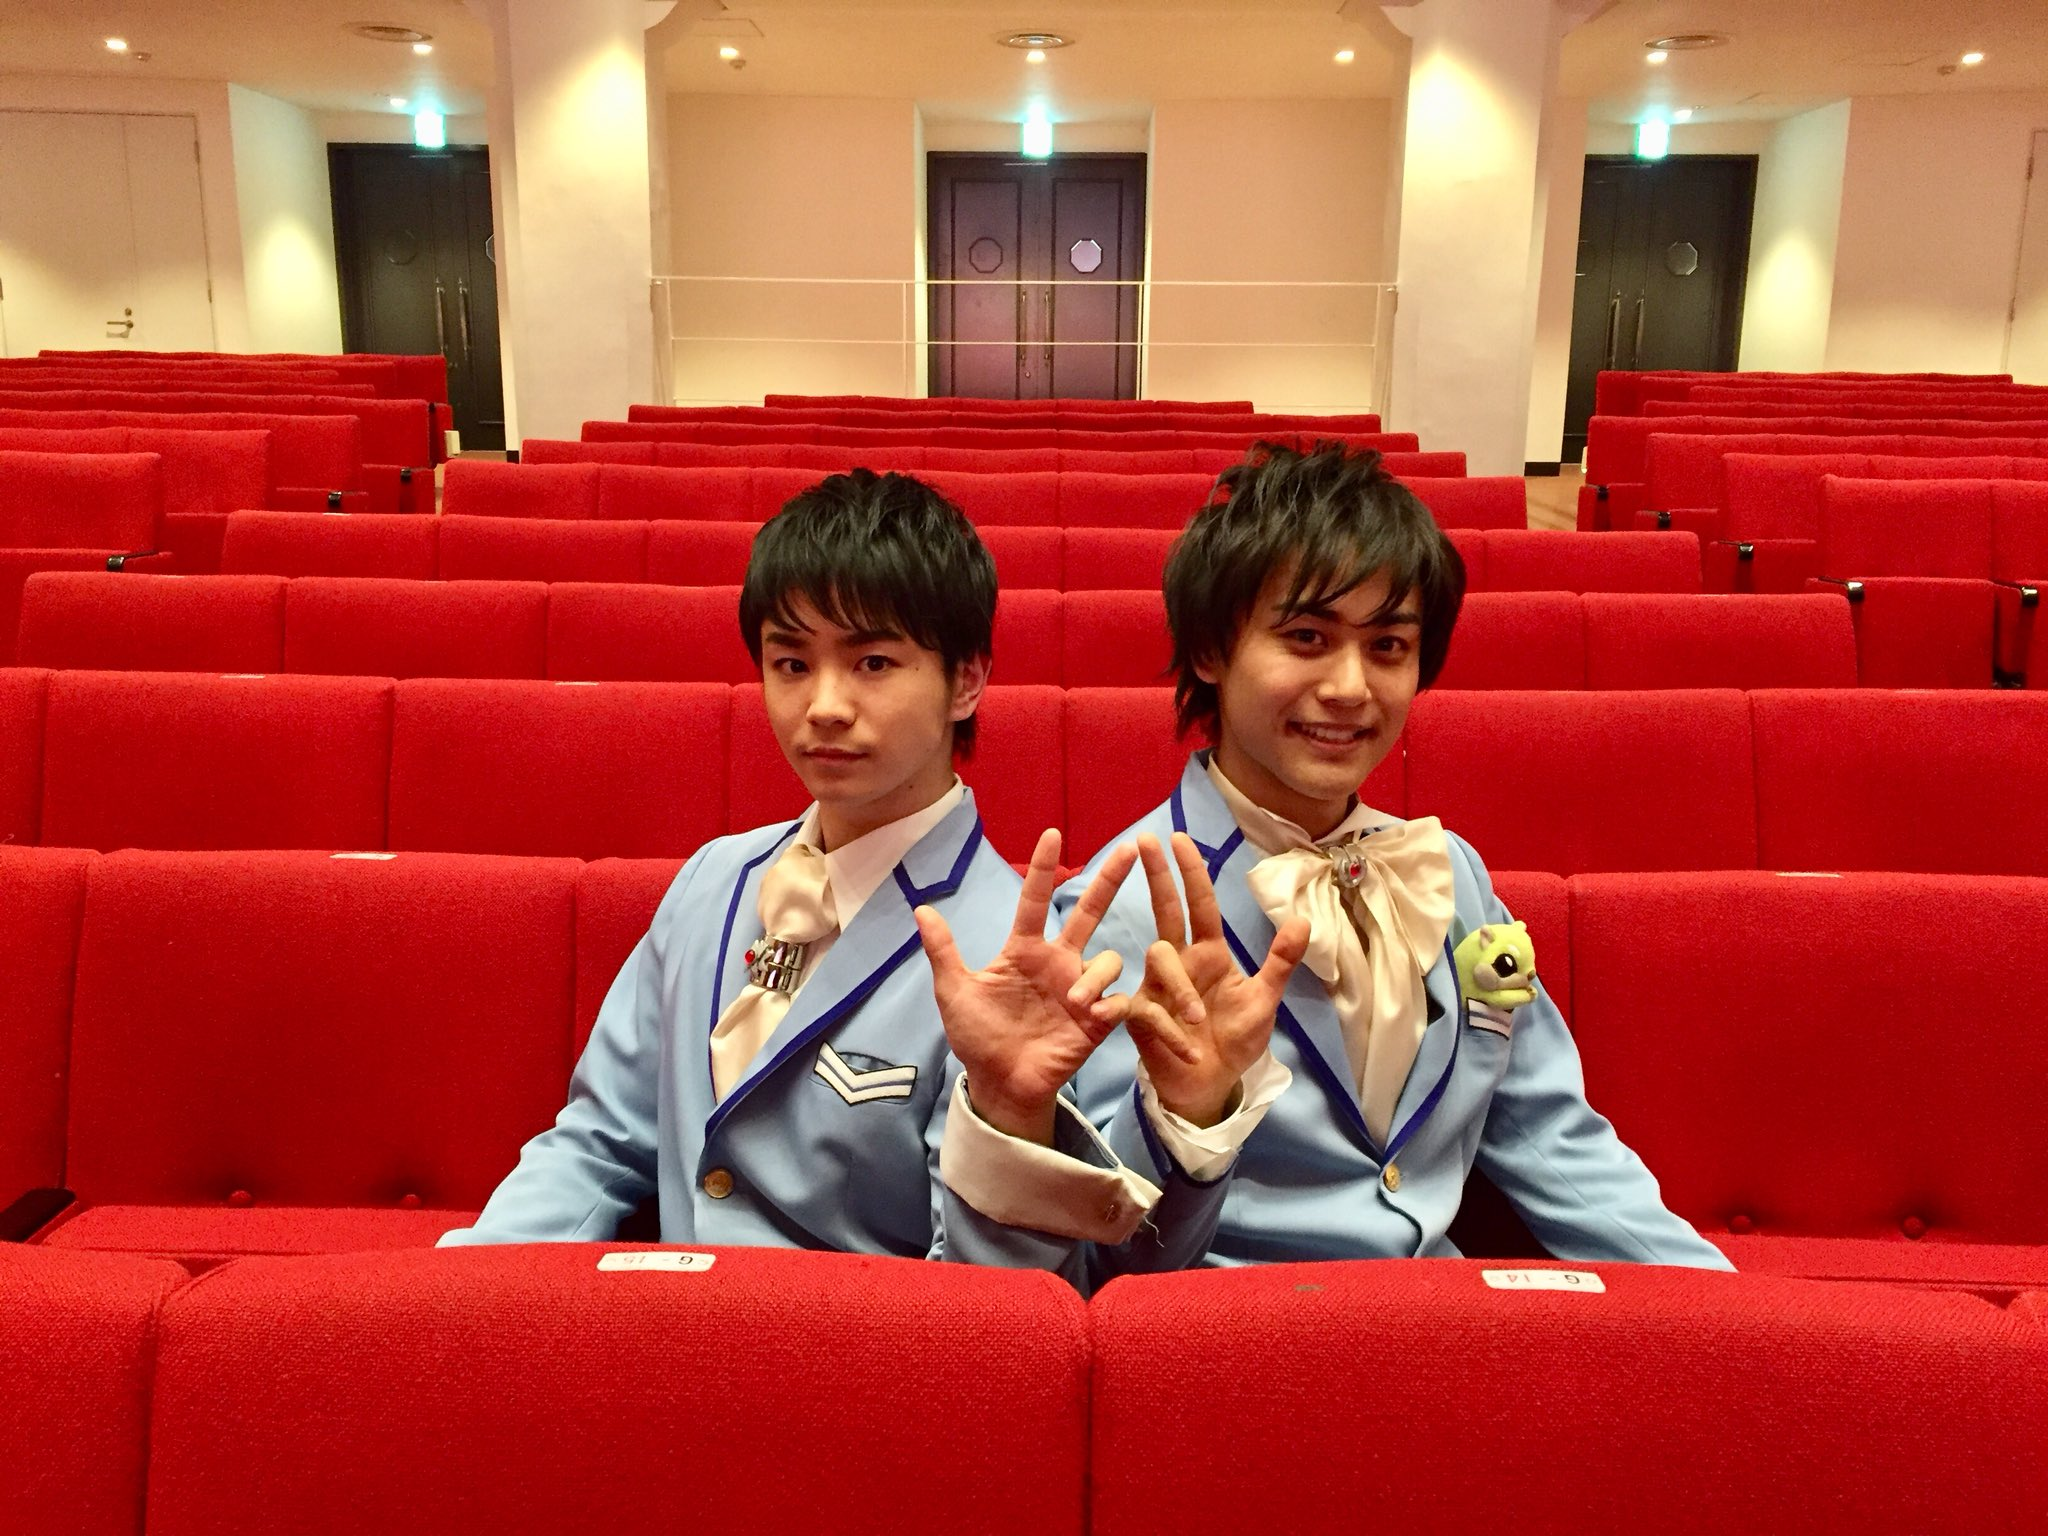
\includegraphics[keepaspectratio,scale=0.05]{fig/dammy.jpg}
\caption{dammy}
\label{dammy}
\end{center}
\end{figure}

\item 位相差を用いた光Race logic回路\\
図()に位相差を用いた光Race logic回路のセル構造を示す.
また,カウンタではアレイに出力された光伝搬信号の位相を計測する.
\begin{figure}[t!]
\begin{center}
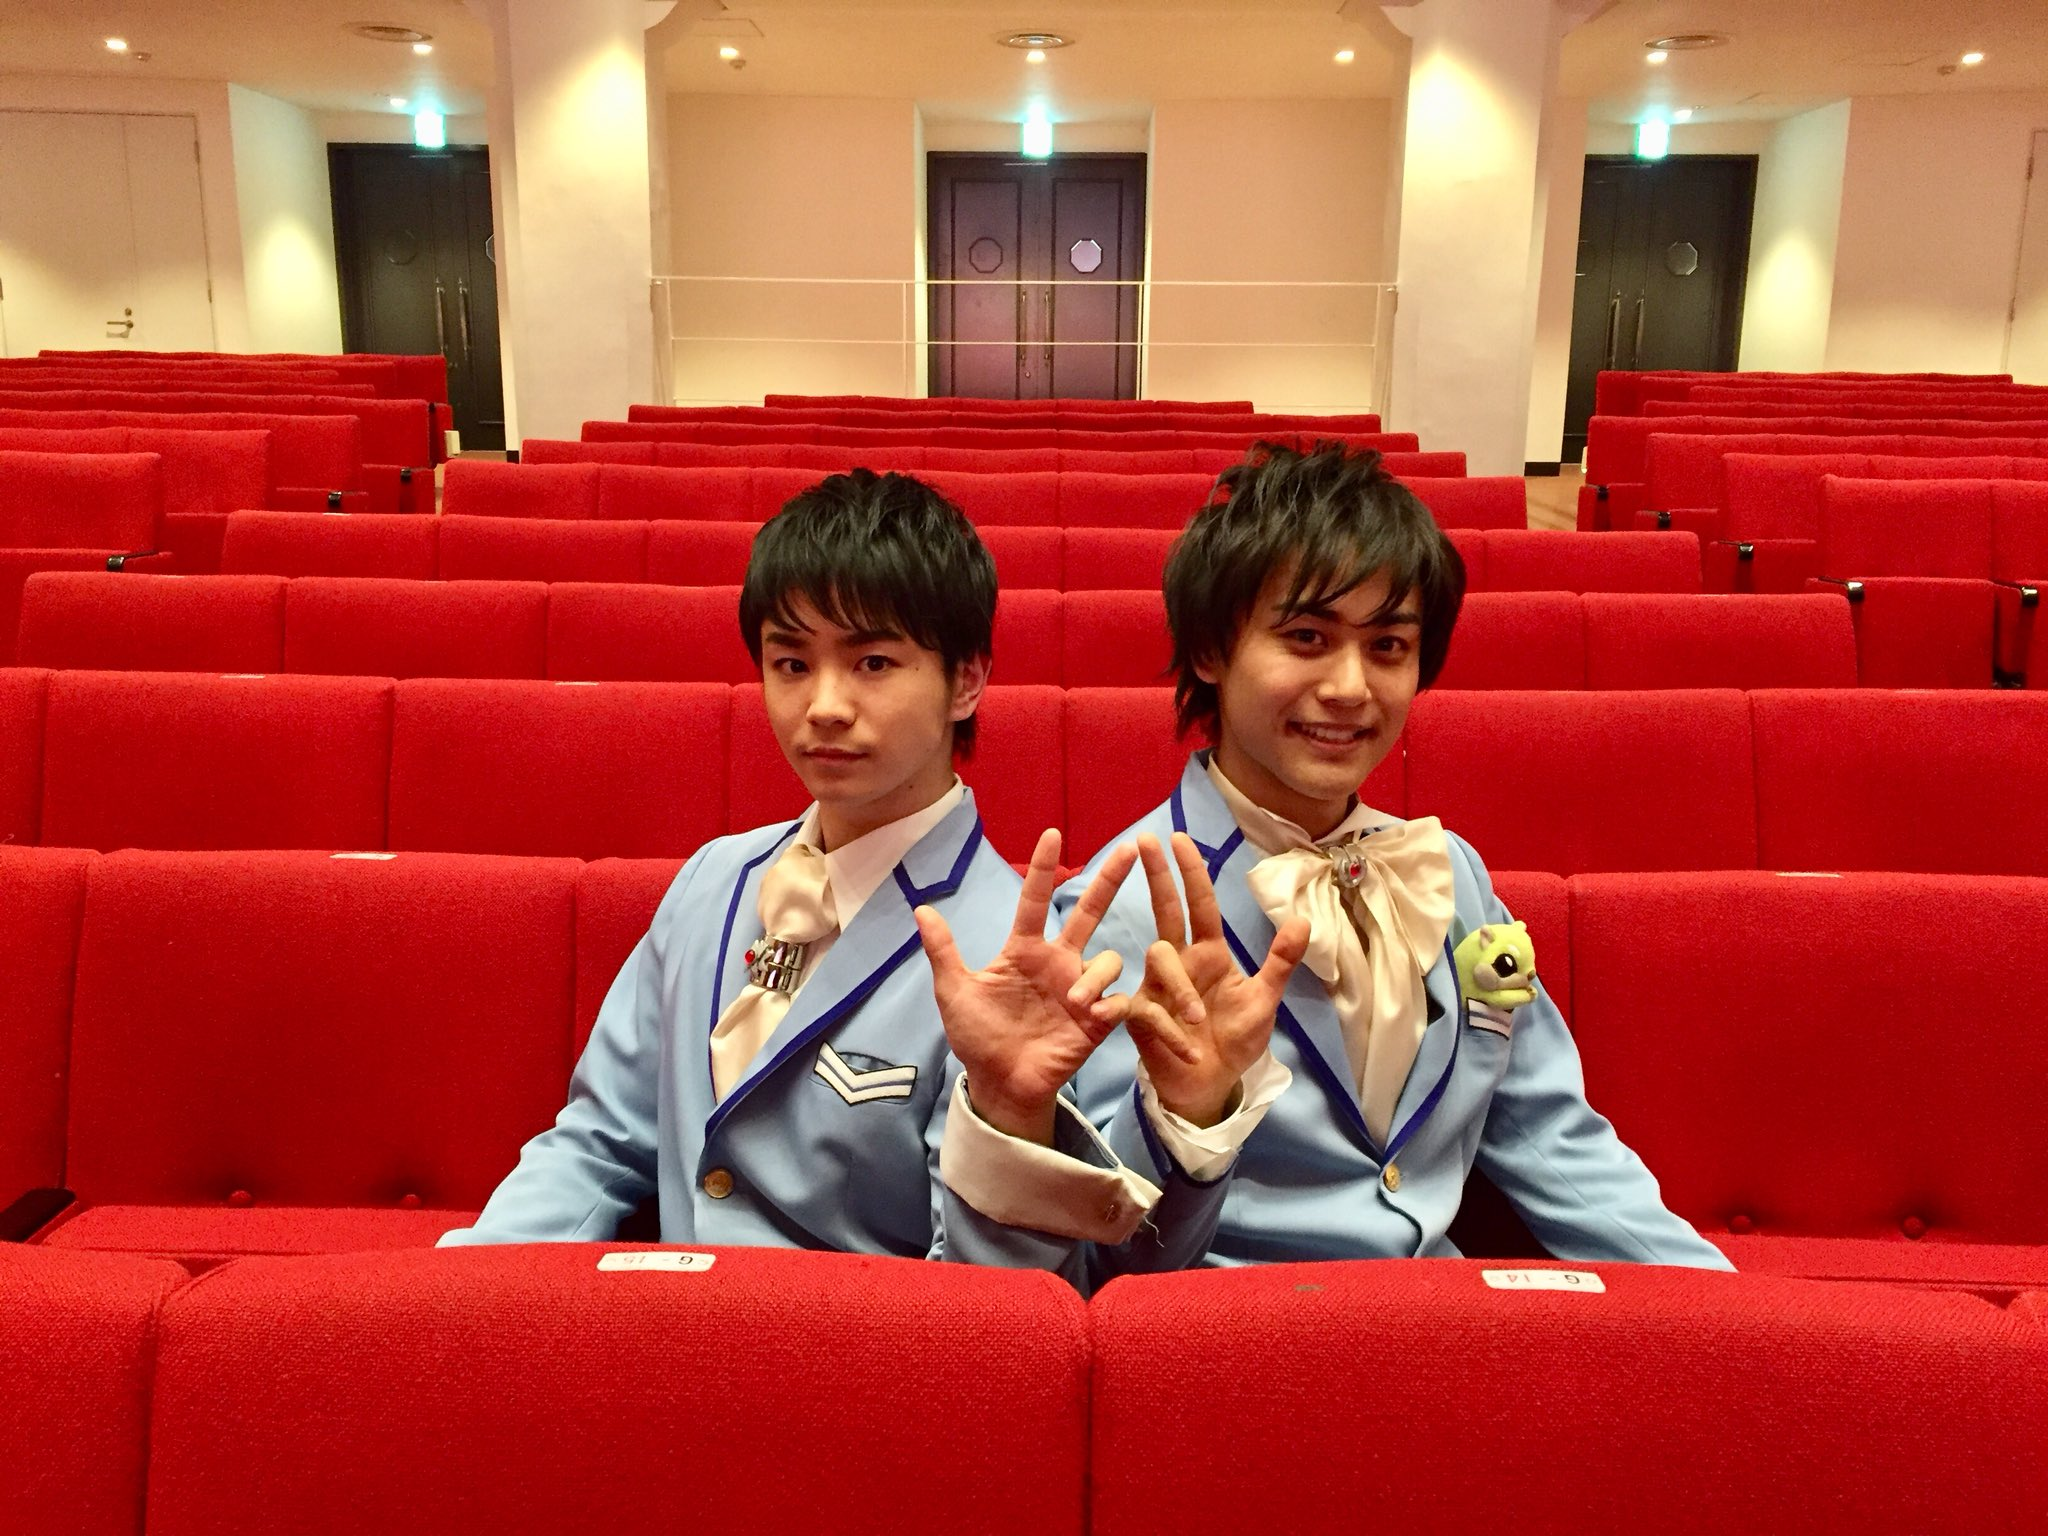
\includegraphics[keepaspectratio,scale=0.05]{fig/dammy.jpg}
\caption{dammy}
\label{dammy}
\end{center}
\end{figure}

\item 伝搬信号強度差を用いた光Race logic回路\\
図()に伝搬信号強度差を用いた光Race logic回路のセル構造を示す.
また,カウンタではアレイに出力された光伝搬信号の信号強度を計測する.
\begin{figure}[t!]
\begin{center}
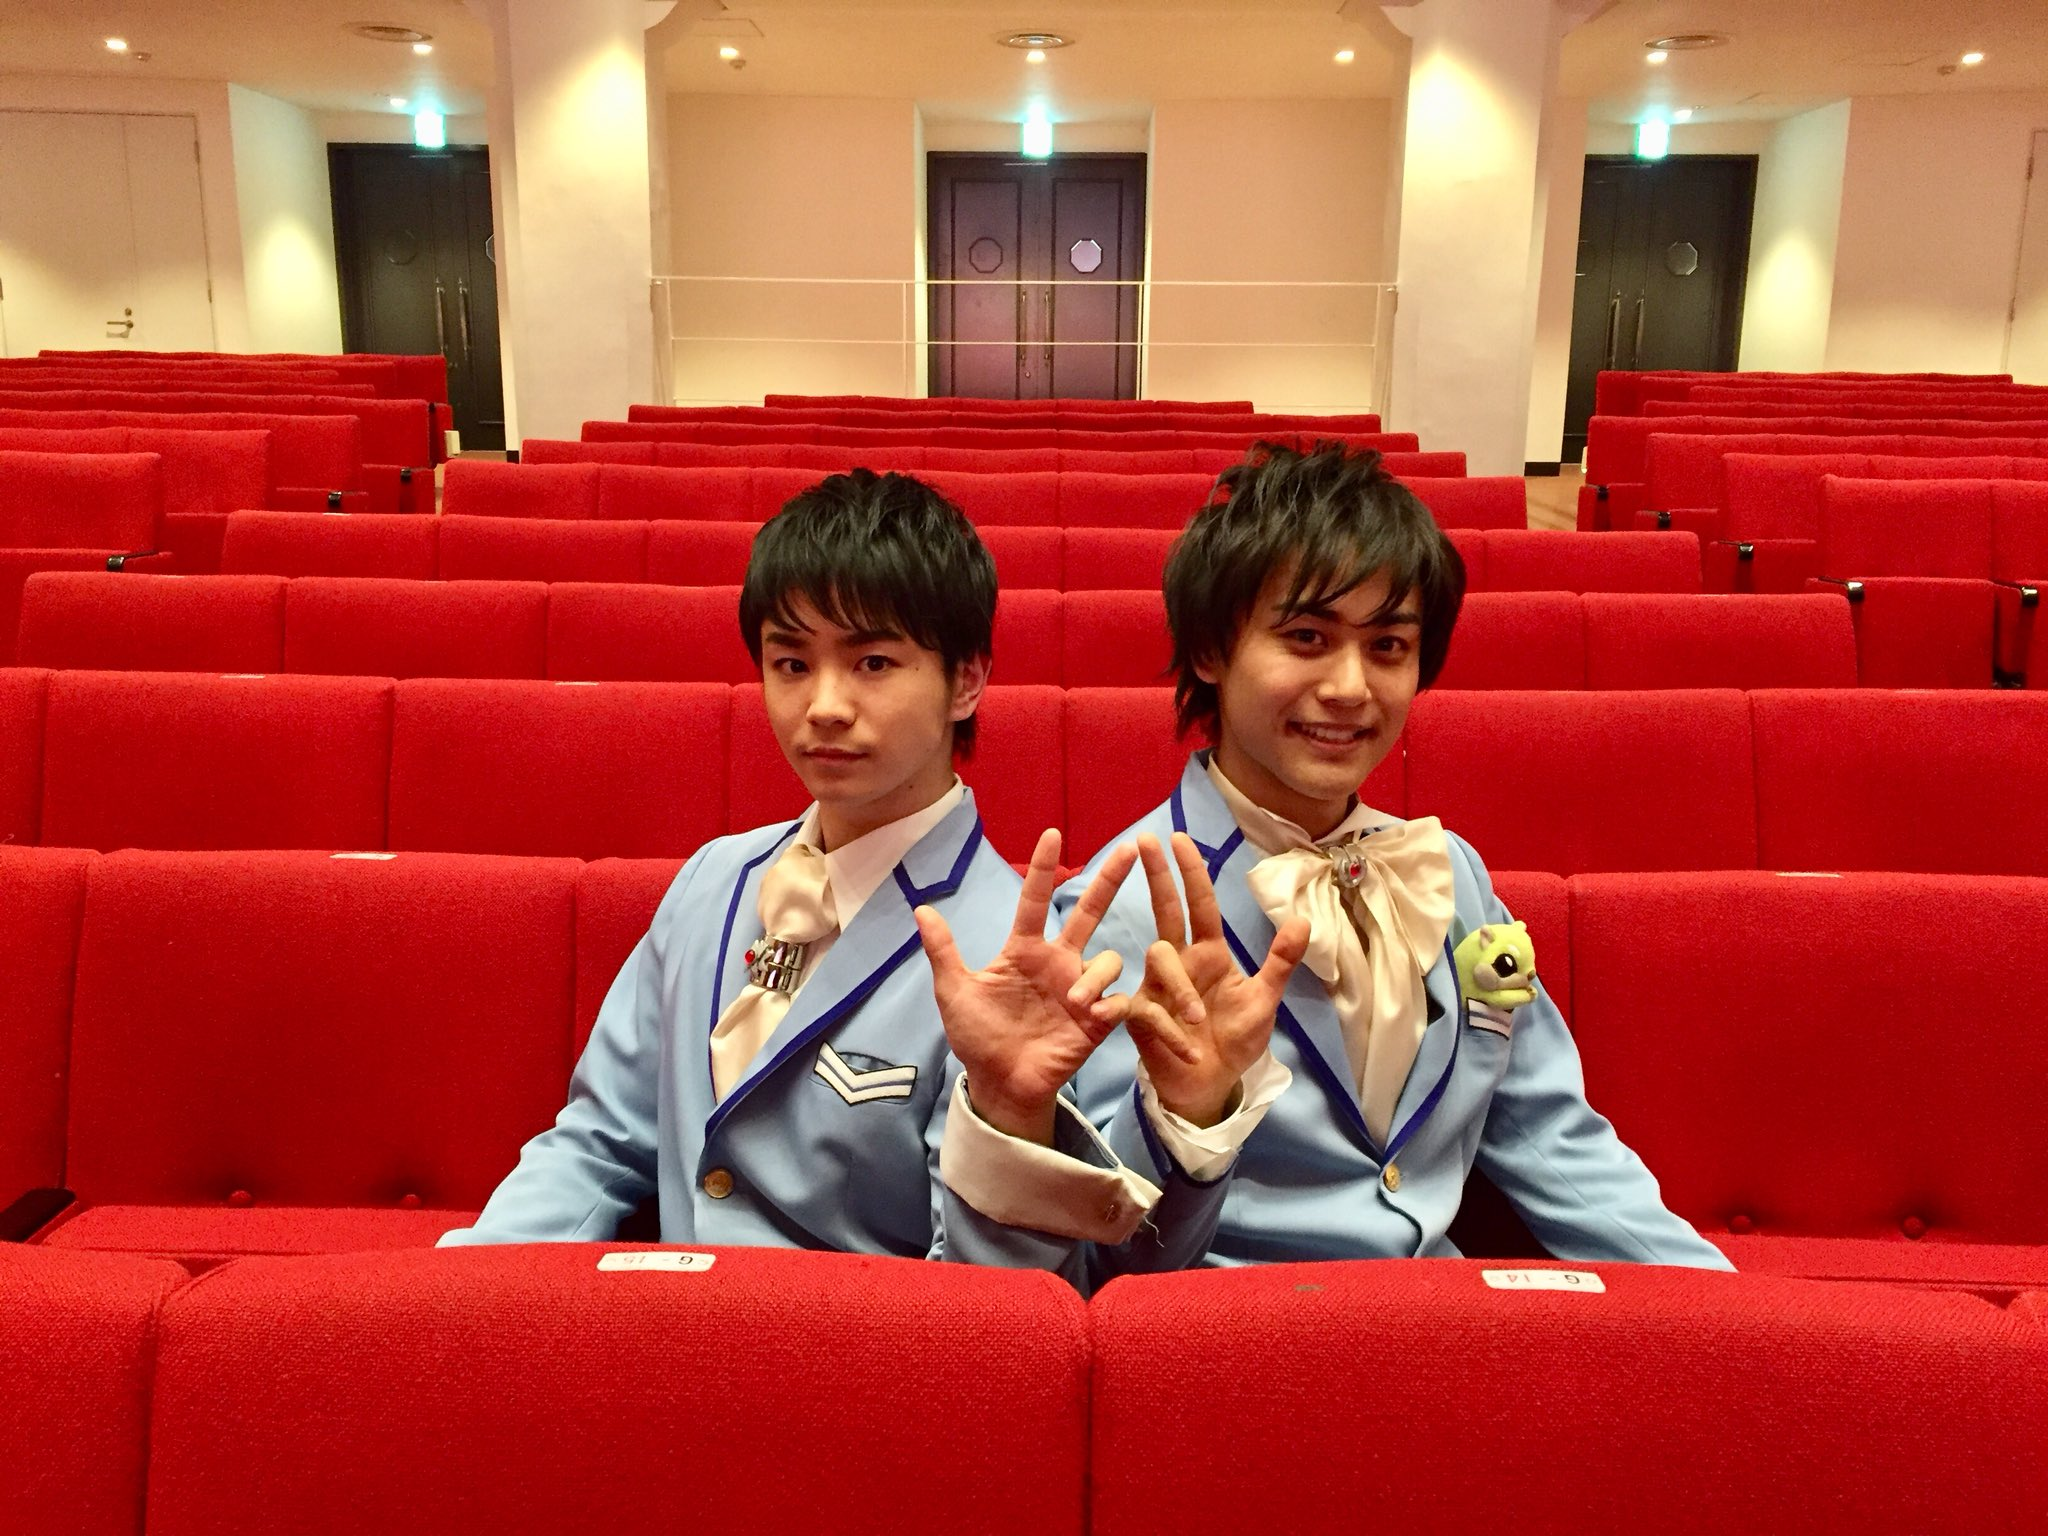
\includegraphics[keepaspectratio,scale=0.05]{fig/dammy.jpg}
\caption{dammy}
\label{dammy}
\end{center}
\end{figure}

\end{itemize}

提案した3つの回路について,次章にて検証・評価を行う.

